This chapter discusses quotient types defined as widely understood traces of normalization functions. The inductive types presented here are inspired by how normalization works for selected quotient types. Some examples reinvented in this chapter are commonly used in Coq, and some are new construction created for this thesis.
\section{Free monoids}
\begin{defi}{Monoid}{def:monoid}
A algebraic structure $(\mathbf{A}, \circ)$, where $\mathbf{A}$ is a carrier set and $\circ: \mathbf{A} \rightarrow  \mathbf{A} \rightarrow \mathbf{A}$ is binary operation is a \emph{monoid} \cite{AbstractAlgebra} if:
\setlist{nolistsep}
\begin{itemize}
    \itemsep 0em 
    \item exists neutral element e $\in \mathbf{A}$, such that $\forall x \in \mathbf{A}. e \circ x = x = x \circ e$,
    \item the binary operation $\circ: \mathbf{A} \rightarrow  \mathbf{A} \rightarrow \mathbf{A}$ is associative, that means $\forall x, y, z \in \mathbf{A}. x \circ (y \circ z) = (x \circ y) \circ z$.
\end{itemize}
\end{defi}
\begin{example}{Monoid of single argument functions}{ex:funcMonoid}
An algebraic structure of single argument functions with function composition operation is an example of a monoid. Function composition is an associative operation, and identity function is a neutral element of this monoid.
\end{example}
\begin{defi}{Free object}{def:freeObject}
\emph{Free object} $\mathbf{A}$ over algebraic structure is the object where the only equations that hold between elements of the free object are those that follow from the defining axioms of the algebraic structure \cite{AbstractAlgebra}.
\end{defi}
\begin{vis}{Equivalent monoids}{vis:equiv_monoids}
Two equivalent free monoids notations of $a \circ b \circ c \circ d$.
\begin{center}
\begin{tikzpicture}[sibling distance=24pt]
    \tikzset{level distance=60pt}
    \Tree [.$\circ$ [.$\circ$ a b ] [.$\circ$ c d ] ]
    \end{tikzpicture}
    \hspace{1cm}
    \begin{tikzpicture}[sibling distance=24pt]
    \Tree [.$\circ$ a [.$\circ$ b [.$\circ$ c [.$\circ$ d e ] ] ] ]
    \end{tikzpicture}
\end{center}
\end{vis}
\begin{example}{Free monoid}{ex:freeMonoid}
Lists of natural numbers are a great example of free monoids. Lists, in general, are often called free monoids. We can concatenate lists of natural numbers using the monoid binary operation $\circ$. By associativity order of concatenation operation does not matter. The neutral element can be used as an empty list. Since this structure is free, we do not worry about the properties of the carrier set.
$$(1 \circ 2) \circ (e \circ 3) = (1 \circ 2) \circ 3 =  1 \circ 2 \circ 3 \not= 6$$
\end{example}
\subsection{A naive representation}
We are accustomed to list representation of free monoids. However, not every notation of free monoids can be expressed in this form. We call the type of every notation of free monoid a naive representation. A first attempt to implement free monoid in Coq for someone unfamiliar with this concept would likely look similar. 
\begin{defi}{Naive free monoid}{def:naiveMonoid}
\begin{minted}{coq}
Inductive FreeMonoid (A: Type) :=
| leaf : FreeMonoid A
| var  : A -> FreeMonoid A
| op   : FreeMonoid A -> FreeMonoid A -> FreeMonoid A.
\end{minted}
\end{defi}
As we can see in the definition above, we have three constructors, an empty list constructor \mcoq{leaf}, a singleton constructor \mcoq{var}, and a list concatenation constructor \mcoq{op}. 
\subsection{The normalized representation}
As it is easy to notice, naive representation \ref{def:naiveMonoid} is not unique for every free monoid, for example, infinitely many representations of the neural element: \mcoq{leaf}, \mcoq{op leaf leaf} etc. To deal with this problem, we must define a normalized free monoid form. For this purpose, we define the following form as normalized:
$$
    (a_1 \circ (a_2 \circ (a_3 \circ \dots  \circ (a_n \circ e) \dots ))
$$
As expected, we devised a classic list representation of free monoid. 
\begin{defi}{List as free monoid}{def:list}
\begin{minted}{coq}
Inductive list (A: Type) :=
| nil  : list A
| cons : A -> list A -> list A.
\end{minted}
\end{defi}
The normalization function finds the first element in the naively defined free monoid, put it as the first constructor, and recursively normalize the rest of the free monoid. If the free monoid is equivalent to a neutral element, the normalization function returns a natural element. The formal definition of this function is not very educative. Therefore we will skip it. However, we will present a conversion function from a naive representation to a normalized one.
\begin{func}{A naive representation to a list conversion}{fn:free_to_list}
\begin{minted}{coq}
Fixpoint free_to_list {A: Type} (m: FreeMonoid A) : list A :=
match m with
| leaf   => []
| var x  => [x]
| op x y => to_list x ++ to_list y
end.
\end{minted}
\end{func}
\section{Integers}
Integers are another classic quotient type with many applications in computer science. They result from extending natural numbers to an additive group by adding an opposite element to every natural number. They can be naively represented as pair of two natural numbers. The first number represents the number of predecessors, and the second represents the number of successors applied to zero.
\subsection{A naive representation}
\begin{defi}{Naive integers representation}{def:naiveInt}
\begin{minted}{coq}
Definition Int : Type := nat * nat.
\end{minted}
\end{defi}
For this representation, we can easily define the addition function by adding the number of predecessors and successors of two numbers.
\begin{func}{Addition of naive integers}{fn:int_add}
\begin{minted}{coq}
Definition int_add (n m: Int) : Int :=
  let (a, b) := n in let (c, d) := m in (a + c, b + d).
\end{minted}
\end{func}
Despite many advantages, this representation is rarely used due to a lack of unique representations. As it is easy to notice, there are infinitely many representations of zero: $1 + (-1)$, $2 + (-2)$, etc. Therefore, we can define a normalization function that will remove redundant pairs of successor and predecessor. After normalization, an integer is made out of eighter predecessors or successors.
\begin{func}{Normalization of naive integers}{fn:int_norm}
\begin{minted}{coq}
Fixpoint int_norm' (x y : nat) : (nat * nat) :=
  match x, y with
  | S x', S y' => int_norm' x' y'
  | _, _       => (x, y)
  end.

Definition int_norm (p: Int) : Int := 
  let (x, y) := p in int_norm' x y.
\end{minted}
\end{func}
\subsection{The normalized representation}
Having a normalization function for our naive representation, we can, based on this normalization process, define an inductive type of normalized representation. The trace of this normalization process is not very interesting until the last recursion. The length of this process depends entirely on how far from the normalized representation the number is. The last step of the normalization process is in function \ref{fn:int_norm} simplified to \mcoq{_, _}. However, we can expand this to three distinct cases:
\begin{description}
\item[\mcoq{S x', O}] -- for negative \mcoq{S x'},
\item[\mcoq{O, S y'}] -- for positive \mcoq{S y'},
\item[\mcoq{O, O}] -- for zero.
\end{description}
Using this trace, we can define the following inductive type for integers. It is a representation known from Coq's standard library \cite{coqDoc}.
\begin{defi}{Normalized integers representation}{def:Z}
\begin{minted}{coq}
Inductive Z : Type :=
| Pos  : nat -> Z
| Zero : Z
| Neg  : nat -> Z.
\end{minted}
\end{defi}
We can also modify a normalization function \ref{fn:int_norm} to convert naive representations into normalized ones.
\begin{func}{Integers conversion}{fn:int_to_Z}
\begin{minted}{coq}
Fixpoint int_to_Z (x y : nat) : Z :=
  match x, y with
  | S x', S y' => int_to_Z x' y'
  | S x', O    => Neg x'
  | O   , S y' => Pos y'
  | O   , O    => Zero
  end.
\end{minted}
\end{func}
\subsection{Basic operations}
We define some basic operations for the normalized representation of integers \ref{def:Z}. Like natural numbers, starting with successor and predecessor definitions is the best option.
\begin{func}{Successor}{fn:int_succ}
\begin{minted}{coq}
Definition succ (n: Z) : Z :=
  match n with
  | Pos k     => Pos (S k)
  | Zero      => Pos O
  | Neg O     => Zero
  | Neg (S n) => Neg n
end.
\end{minted}
\end{func}
\begin{func}{Predecessor}{fn:int_pred}
\begin{minted}{coq}
Definition pred (n: Z) : Z :=
  match n with
  | Pos (S n) => Pos n
  | Pos O     => Zero
  | Zero      => Neg O
  | Neg n     => Neg (S n)
end.
\end{minted}
\end{func}
Both definitions are straightforward but substantially more complicated than the same operations for naive representations. A fourth case was required to handle the transition to zero in both cases.
\begin{func}{Negation}{fn:int_neg}
\begin{minted}{coq}
Definition neg (n: Z) : Z :=
match n with
| Pos k => Neg k
| Zero  => Zero
| Neg k => Pos k
end.
\end{minted}
\end{func}
The definition of negation is simple and does not require a discussion. The next basic operation for integers is addition.
\begin{func}{Map $n$ times}{fn:map_n}
\begin{minted}{coq}
Fixpoint map_n {A: Type} (n: nat) (f: A -> A) (x: A) : A :=
  match n with
  | O    => x
  | S n' => f (map_n n' f x)
  end.
\end{minted}
\end{func}
  
\begin{func}{Addition}{fn:Z_add}
\begin{minted}{coq}
Definition add (a b : Z) : Z :=
  match a with 
  | Pos n => map_n (S n) succ b
  | Zero  => b
  | Neg n => map_n (S n) pred b
  end.
\end{minted}
\end{func}
For defining addition, we first needed to define an ancillary function that applies some function $n$ times. Using it, we can define addition as applying the successor operation several times. Subtraction can be defined as the addition of an opposite number.
\begin{func}{Multiplication}{fn:int_mul}
\begin{minted}{coq}
Definition mul (a b: Z) : Z :=
  match a with 
  | Pos n => map_n (S n) (add b) Zero
  | Zero  => Zero
  | Neg n => neg (map_n (S n) (add b) Zero)
  end.
\end{minted}
\end{func}
The multiplication operation can be defined as adding the same number several times. As we know, the addition and multiplication of integers are commutative and associative. Moreover, multiplication is distributive over addition. Proofs of those facts are too long to be presented in this paper. Thou, they can be in \coqsource{Integers.v}.
\section{Exotic integers}
Integers defined in the previous section are a great choice due to their symmetric simple definition and computational properties. For example, the addition has linear complexity to one of the arguments. A small detail that leaves a bad taste is that we used inductive type of natural numbers in the definition of integers. The question arises if there is a definition of integers that uses a single inductive type.

\subsection{The alternative normalized representation}
We can define the normalization process in an alternative way. Instead of finishing when we determine if the number is positive or negative, we can continue the process by moving successors from input to output. Of course, this step is de facto an identity function on natural numbers with linear complexity.
\begin{func}{Alternative normalization}{fn:int_alt_norm}
\begin{minted}{coq}
Fixpoint alt_norm (n m: nat) : nat * nat :=
  match n, m with
  | S n', S m' => alt_norm n' m'
  | O   , S _  => map_n n 
      (fun (i: nat * nat) => let (x, y) := i in (S x, y)) (O, O)
  | O   , _    => map_n m 
      (fun (i: nat * nat) => let (x, y) := i in (x, S y)) (O, O)
  end.
\end{minted}
\end{func}
This unnecessary step changes the trace of the normalization process. Now, after determining the sign of the integer, the length of the trace defines its value. This part of the trace is almost identical for positive and negative numbers. Therefore, they will both use a single constructor \mcoq{Next}. We will use two different nullary constructors for parts of traces when the integer sign is determinate, named \mcoq{Zero} and \mcoq{MinusOne}.
\begin{defi}{Exotic integers representation}{def:Z'}
\begin{minted}{coq}
Inductive Z' : Type :=
| Zero     : Z'
| MinusOne : Z'
| Next     : Z' -> Z'.
\end{minted}
\end{defi}
The \mcoq{Next} constructor is both successor and predecessor depending on the integer on which it is applied. On a negative integer, it is a predecessor; on a zero or positive number, it is a successor. This representation is uncommon. We could not find any paper or document that used it. Most likely, since the definition from the previous section meets almost all criteria for perfect integers representation.
\begin{func}{Conversion to exotic integrs}{fn:to_Z'}
\begin{minted}{coq}
Fixpoint to_Z' (n m: nat) : Z' :=
  match n, m with
  | S n', S m' => to_Z' n' m'
  | O   , S m' => map_n m' Next MinusOne
  | _   , O    => map_n n Next Zero
  end.
\end{minted}
\end{func}
\subsection{Basic operations}
This definition of integers, however, could be more convenient for defining operations. As we can notice, to determine the sign of a number, we need to check the last constructor. Since our definition uses this same construction for successor and predecessor, even a simple operation of computing the successor of a number has linear complexity.
\begin{func}[D]{Successor}{fn:Z'_succ}
\begin{minted}{coq}
Fixpoint succ (k : Z') : Z' :=
  match k with
  | Zero => Next Zero
  | MinusOne => Zero
  | Next Zero => Next (Next Zero)
  | Next MinusOne => MinusOne
  | Next k' => Next (succ k')
  end.
\end{minted}
\end{func}
\begin{func}{Predecessor}{fn:Z'_pred}
\begin{minted}{coq}
Fixpoint pred (k : Z') : Z' :=
  match k with
  | Zero => MinusOne
  | MinusOne => Next MinusOne
  | Next Zero => Zero
  | Next MinusOne => Next (Next MinusOne)
  | Next k' => Next (pred k')
  end.
\end{minted}
\end{func}
Because of those difficulties, we recommend using an intermediate form of naively defined integers \ref{def:naiveInt} or the previous normalized definition of integers representation \ref{def:Z} to carry out computations. The conversion functions can be easily defined. The proof of standard and exotic integers definitions being isomorphic with some proofs of basic properties for exotic integers can be found in \coqsource{ExoticInteger.v}.
\section{Positive rational numbers}
In contrast to integers coming up with a type for rational numbers with unique representation is a challenging task. This section is based on the work of Yves Bertot \cite{Qplus}, which presents a solution to this problem based on a trace of the Euclidean algorithm.
\subsection{A naive representation}
A naive representation of positive rational numbers is identical to that of integers. It comprises two natural numbers, one for a numerator and one for a denominator. Of course, we cannot divide by zero. Therefore we can interpret the second number predecessor of the denominator or accept that some pairs do not represent any number.
\begin{defi}{Naive representation of rational numbers }{def:naiveQ}
\begin{minted}{coq}
Definition Q' : Type := nat * nat.
\end{minted}
\end{defi}
We chose the second option since we want to use an already defined coq operation on natural numbers. As we know from mathematics, there are many notations for this same fraction. $\frac{1}{2}$ or $\frac{2}{4}$ represents the same rational number a half. Every fraction can be reduced to a normal irreducible fraction. In order to find this irreducible fraction, we need to divide the numerator and denominator by their greatest common denominator. There are many algorithms to compute this value, but one of the simplest is the Euclidean algorithm.
\begin{func}{Euclidean algorithm}{fn:euclid}
\begin{minted}{coq}
Fixpoint euclid (p q: nat) : nat :=
  match compare p q with
  | Eq => p
  | Gt => euclid (p - q) q n'
  | Lt => euclid p (q - p) n'
  end.
\end{minted}
\end{func}
The Euclidean algorithm is based on the law that states $\textrm{gcd}(a, b) = \textrm{gcd}(a - b, b)$ if $a > b$. The observation that will be important for defining a normalized representation is that the trace of this algorithm is the same if both numbers are multiplied by the same positive natural number, as in the example shown below.
\begin{equation}
    \begin{split}
        11k&>5k\\
        (11-5)k=6k&>5k\\
        (6-5)k=k&<4k\\
        k&<3k=(4-1)k\\
        k&<2k=(3-1)k\\
        k&=k=(2-1)k
    \end{split}
\end{equation}
The trace,  defined as inequality signs between values, does not change and does not depend on chosen value $k$. The other observation is that we can compute the input values by knowing the trace of the Euclidean algorithm and the output. Without the output, we can still compute the proportions of the input value. The proof of those statements can be found in \coqsource{Qplus.v}.
\subsection{The normalized representation}
Based on those observations, we define an inductive type for positive rational numbers. It has three constructors: \mcoq{N} when the nominator was greater, \mcoq{D} when the denominator was greater, and \mcoq{One} when both values were the same.
\begin{defi}{Normalized representation}{def:Qplus}
\begin{minted}{coq}
Inductive Qplus : Type :=
| One : Qplus
| N   : Qplus -> Qplus
| D   : Qplus -> Qplus.
\end{minted}
\end{defi}
This construction also provides a nice induction rule for positive rational numbers. The type \mcoq{Qplus} is based on the Euclidean algorithm. Therefore the conversion function is slightly modified by Euclidean algorithm that, instead of computing the greatest common denominator, returns its trace. 
\begin{func}{Conversion to the Euclid's algorithm trace}{def:qplus_c}
\begin{minted}{coq}
Fixpoint qplus_c' (p q n: nat) : Qplus :=
  match n with
  | O    => One
  | S n' => match compare p q with
            | Eq => One
            | Gt => N (qplus_c' (p - q) q n')
            | Lt => D (qplus_c' p (q - p) n')
            end
  end.

Definition qplus_c (x: Q') : Qplus :=
  let (p, q) := x in qplus_c' p q ((p + q) / gcd p q).
\end{minted}
\end{func}
This function differs from the Euclidean algorithm defined in \ref{fn:euclid} since the Coq's termination checker cannot deduce the decreasing argument. Therefore defining the Euclidean algorithm this way is illegal in Coq (8.14.1). We circumvent this problem by adding an argument (the fuel) that constantly decreases, satisfying the termination condition. In order to not change the algorithm output, we need to set the fuel to be big enough. We know that the Euclidean algorithms need fewer steps to compute the result than the sum of its inputs. Moreover, as we noticed, multiplying inputs by positive numbers does not change the computations so that we can divide the fuel by the greatest common denominators of inputs.
\begin{func}{Conversion to naive representation}{def:qplus_i}
\begin{minted}{coq}
Function qplus_i (x : Qplus) : Q' :=
  match x with
  | One  => (1, 1)
  | N x' => let (p, q) := qplus_i x' in (p + q, q)
  | D x' => let (p, q) := qplus_i x' in (p, p + q)
  end.
\end{minted}
\end{func}
The inverse conversion function is an even simpler construction. It is based on $(p - q) + q = p$. Of course, the inverse function does not return the same fraction but the equivalent irreducible fraction. The proof that this functions are inversions up to equivalency can be found in \coqsource{Qplus.v}
\subsection{Extension to the field of rational numbers}
There is a  natural extension to the field of rational numbers. It uses this same construction as the extension of natural numbers to integers (see \ref{def:Z}).
\begin{defi}{Type of normalized rational numbers}{def:FullQ}
\begin{minted}{coq}
Inductive FullQ :=
| QPos  : Qplus -> FullQ
| QZero : FullQ
| QNeg  : Qplus -> FullQ.
\end{minted}
\end{defi}
This type uses defined in this section traces of Euclidean algorithm as the normalized representation of a positive rational number. Therefore, we can extend most of the theorems defined for positive rational numbers to the field extension.
\subsection{Basic operations}
In the field of rational numbers, we can define basic operations. However, the proposed normalized representation is not suited for computations. Therefore will define computations in the homomorphic representation using pair of two integers. However, only a fraction with positive denominators represents a valid rational number.
\begin{defi}{Type of naive rational numbers}{def:Q}
\begin{minted}{coq}
Definition Q : Type := Z * Z.
\end{minted}
\end{defi}
In order to use it to perform computations, we also need to define conversion functions.
\begin{func}{Absolute value}{fn:abs'}
\begin{minted}{coq}
Definition abs' (n: Z) : nat :=
  match n with
  | Pos k => S k
  | Zero => O
  | Neg k => S k
  end.
\end{minted}
\end{func}
\begin{func}{Embedding natural numbers into integers}{fn:toPos}
\begin{minted}{coq}
Definition toPos (x: nat) : Z :=
  match x with
  | O   => Zero
  | S n => Pos n
  end.
\end{minted}
\end{func}
We first need an integer to the natural number absolute value function \ref{fn:abs'}. And natural number to integer function \ref{fn:toPos}.
\begin{func}{Conversion to the normalized rational number}{fn:fullQ_c}
\begin{minted}{coq}
Definition fullQ_c (q: Q') : FullQ :=
  match q with
  | (Pos n, d) => QPos (qplus_c (S n, abs' d))
  | (Zero , d) => QZero
  | (Neg n, d) => QNeg (qplus_c (S n, abs' d))
  end.
\end{minted}
\end{func}
The conversion function \ref{fn:fullQ_c} works only for fractions with a positive denominator.
\begin{func}{Conversion to the naive rational number}{fn:fullQ_i}
\begin{minted}{coq}
Definition fullQ_i (q: FullQ) : Q :=
  match q with
  | QPos q' => let (n, d) := qplus_i q' in (toPos n, toPos d)
  | QZero   => (Zero, Pos O)
  | QNeg q' => let (n, d) := qplus_i q' in (-toPos n, toPos d)
  end.
\end{minted}
\end{func}
The inverse conversion function \ref{fn:fullQ_i} produces an irreducible fraction with a positive denominator. Having all conversion functions, we can define the addition operation.
\begin{func}{Addition}{fn:Qadd}
\begin{minted}{coq}
Definition Qadd' (x y: Q') : Q' :=
  match x, y with
  | (n, d), (n', d') => (d' * n + d * n', d * d')
  end.

Definition Qadd (x y: FullQ) : FullQ :=
  fullQ_c (Qadd'(fullQ_i x) (fullQ_i y)).
\end{minted}
\end{func}
The additional operation adds numerators of two fractions reduced to a common denominator.
\begin{func}{Negation}{fn:Qneg}
\begin{minted}{coq}
Definition Qneg (q: FullQ) : FullQ :=
  match q with
  | QPos x => QNeg x
  | QZero  => QZero
  | QNeg x => QPos x
  end.
\end{minted}
\end{func}
The negation switches the sign of a rational number. Subtraction can be defined as the addition of a negative number.
\begin{func}{Multiplication}{fn:Qmul}
\begin{minted}{coq}
Definition Qmul' (x y: Q') : Q' :=
  match x, y with
  | (n, d), (n', d') => (n * n', d * d')
  end.

Definition Qmul (x y: FullQ) : FullQ :=
  fullQ_c (Qmul' (fullQ_i x) (fullQ_i y)).
\end{minted}
\end{func}
The multiplication operation multiplies both numerators and denominators.
\begin{func}[D]{Inversion}{fn:Qinv}
\begin{minted}{coq}
Fixpoint Qplus_inv (q: Qplus) : Qplus :=
  match q with
  | N x => D (Qplus_inv x)
  | One => One
  | D x => N (Qplus_inv x)
  end.

Definition Qinv (q: FullQ) : FullQ :=
  match q with
  | QPos x => QPos (Qplus_inv x)
  | QZero  => QZero
  | QNeg x => QNeg (Qplus_inv x)
  end.
\end{minted}
\end{func}
The inversion can be easily computed on the Euclidean algorithm trace by swapping two constructors \mcoq{N} and \mcoq{D}. As we know, the inverse operation switches the numerator and the denominator. By swapping inputs of the Euclidean algorithm, we changed which number was bigger at all steps. The division can be defined as multiplying the inversion. The proof that rational numbers with those operations are an algebraic field can be found in \coqsource{Extras/FullQ.v}.
\section{Free groups}
In this chapter, we learned how to define a free monoid; in this section, we define another free algebraic structure -- a free group.
\begin{defi}{Group}{def:group}
A algebraic structure $(\mathbf{A}, \circ)$, where $\mathbf{A}$ is a carrier set and $\circ: \mathbf{A} \rightarrow  \mathbf{A} \rightarrow \mathbf{A}$ is binary operation is a \emph{group} \cite{AbstractAlgebra} if:
\setlist{nolistsep}
\begin{itemize}
    \itemsep 0em 
    \item exists neutral element e $\in \mathbf{A}$, such that $\forall x \in \mathbf{A}. e \circ x = x = x \circ e$,
    \item the binary operation $\circ: \mathbf{A} \rightarrow  \mathbf{A} \rightarrow \mathbf{A}$ is associative, that means $\forall x, y, z \in \mathbf{A}. x \circ (y \circ z) = (x \circ y) \circ z$.
    \item for every element $x$ there is an inverse element $x^{-1}$, such that $x \circ x^{-1} = x^{-1} \circ x = e$.
\end{itemize}
\end{defi}
\begin{example}{Group of permutations}{ex:permutations}
An interesting example is a group of permutations $S_n$, with permutations composition as a binary operation. The composition of the function (permutation is a function), as we learned in the example of monoid \ref{ex:funcMonoid} is associative. The constant permutation is the neutral element. We can compute inverse permutation by swapping inputs with outputs for every permutation.
$$
\begin{pmatrix}
    1 & 2 & 3 & 4 & 5 \\
    2 & 3 & 1 & 5 & 4
\end{pmatrix}^{-1}
=
\begin{pmatrix}
    1 & 2 & 3 & 4 & 5 \\
    3 & 1 & 2 & 5 & 4
\end{pmatrix}
$$
\end{example}
\subsection{A naive representation}
We know that a free monoid can be represented as a list. The difference between a monoid and a group is the existence of inverse elements. Therefore we can naively define a free monoid as a list of elements and the sign (information if the element is inverted or not) of the element.
\begin{defi}{Naive free group representation}{def:CanonFreeGroup}
\begin{minted}{coq}
Definition NaiveFreeGroup (A: Type) := list (bool * A).
\end{minted}
\end{defi}
As it is easy to notice, this representation is not unique for every free group. Therefore we need to define a normalization function. In our case, we will reduce two elements next to each other but with opposite signs to a neutral element (empty list).
\begin{defi}{Normalized naive representation}{def:Normalized}
\begin{minted}{coq}
Inductive Normalized {A: Type} : NaiveFreeGroup A -> Prop :=
| NNil   : Normalized []
| NSingl : forall (b : bool) (v : A), Normalized [(b, v)]
| NCons  : forall (b b': bool) (v v' : A) (x: NaiveFreeGroup A), 
            v <> v' \/ b = b' -> Normalized ((b', v') :: x) ->
            Normalized ((b, v) :: (b', v') :: x).
\end{minted}
\end{defi}
We need an underlying type with decidable equality to define the normalization function.
\begin{defi}{Decidable equality in Coq}{def:EqDec}
\begin{minted}{coq}
Class EqDec (A : Type) := { 
  eqf : A -> A -> bool ;
  eqf_leibniz : forall x y: A, reflect (x = y) (eqf x y);
}.
\end{minted}
\end{defi}
\begin{coq}{Reflect}{coq:reflect}
Reflect is an inductive type for
relating propositions and booleans \cite{coqDoc}.
\begin{minted}{coq}
Inductive reflect (P : Prop) : bool -> Set :=
| ReflectT : P -> reflect P true
| ReflectF : (P -> False) -> reflect P false.
\end{minted}
\end{coq}
\begin{func}{Normalization function for free group}{fn:normalize}
\begin{minted}{coq}
Fixpoint normalize {A: Type} `{EqDec A} (x: NaiveFreeGroup A) :=
  match x with
  | [] => []
  | (b, v) :: x' => 
      match normalize x' with
      | [] => [(b, v)]
      | (b', v') :: x'' => 
          if andb (eqf v v') (xorb b b')
          then x''
          else (b, v) :: (b', v') :: x''
      end
  end.
\end{minted}
\end{func}
\subsection{The normalized representation}
Based on the normalization process, we will define an inductive type where two of the same elements with opposite signs cannot be next to each other. In order to define this type, we first need to formalize the group in Coq.
\begin{defi}{Typeclass of groups}{def:coqGroup}
\begin{minted}{coq}
Class Group (A : Type) := GroupDef {
  zero     : A;
  op       : A -> A -> A;
  inv      : A -> A;
  l_op_id  : forall x: A, op zero x = x;
  r_op_id  : forall x: A, op x zero = x;
  l_op_inv : forall x: A, op (inv x) x = zero;
  r_op_inv : forall x: A, op x (inv x) = zero;
  op_assoc : forall x y z: A, op (op x y) z = op x (op y z);
}.

Class EqGroup (A : Type) `{E: EqDec A} `{G: Group A} := {}.

Definition sub {A: Type} `{Group A} (x y: A) := op x (inv y).
\end{minted}
\end{defi}
We can make the following observations if the underlying type is a group. First, we notice that two elements are equal if and only if the difference between them is a neutral element. The second one is that we can define any list as a list of differences between elements. Similar to the normalization process, the list of differences starts with the last element of the free group then differences from the previous elements are added.
\begin{defi}{Normalized representation of free group}{def:Group}
\begin{minted}{coq}
Inductive NEQuotFreeGroup (A: Type) `{EqGroup A} :=
| Singl  : bool -> A -> NEQuotFreeGroup A
| Switch : forall x: A, Squash (x <> zero) -> 
             NEQuotFreeGroup A -> NEQuotFreeGroup A
| Stay   : A -> NEQuotFreeGroup A -> NEQuotFreeGroup A.

Definition QuotFreeGroup (A: Type) `{EqGroup A} 
  := option (NEQuotFreeGroup A).
\end{minted}
\end{defi}
This inductive type \mcoq{NEQuotFreeGroup} of non-empty normalized free groups is made of three constructors. The first constructor \mcoq{Singl} is the constructor of the last element of a free group. The second one \mcoq{Switch} is the most interesting since it prevents the existence of two elements that differ only by a sign next to each other. It adds an element with a sign opposite to the head of the free group by providing a difference from the head and proof that this difference is not a neutral element. This proof is squashed (see \ref{coq:SProp}), so we do not need to worry about its uniqueness. The third one adds an element with this same sign as the head of the free group by providing a difference to the head. This construction cannot be used to define a type of free group with an empty group since we know that the inverse of neutral elements is a neutral element from the group's laws, and our definition requires providing a sign of every element. Therefore to define potentially empty free groups, we need to use a second definition utilizing an option. \mcoq{None} is the empty list constructor. This construction was created for this paper. The definition of groups and free groups is a common problem in Coq \cite{GroupsCoq} \cite{FreeGroupsCoq}. However, no similar definitions were found. 

To apply this construction in practice, it is necessary to define conversion functions since the normalized representation is difficult for users to read and write. Therefore, the best approach is to define a free group in naive representation and convert them to normalized representation.
\begin{func}{Conversion to normalized representation}{fn:to_quot'}
\begin{minted}{coq}
Fixpoint to_quot' {A: Type} `{EqGroup A} (b : bool) (v: A) 
  (x: NaiveFreeGroup A) : NEQuotFreeGroup A :=
  match x with 
  | []             => Singl b v
  | (b', v') :: x' => 
    if eqb b b' 
    then Stay (sub v v') (to_quot' b' v' x')
    else match eqf_leibniz (sub v v') zero with
         | ReflectF _ p => Switch 
             (sub v v') (squash p) (to_quot' b' v' x')
         | _  => (Singl b v) (* invalid *)
         end
end.
\end{minted}
\end{func}
\begin{func}{Conversion to normalized representation}{fn:to_quot}
\begin{minted}{coq}
Definition to_quot {A: Type} `{EqGroup A} 
  (x: NaiveFreeGroup A) : QuotFreeGroup A :=
match x with
| [] => None
| (b, v) :: x' => Some (to_quot' b v x')
end.
\end{minted}
\end{func}
In the definition of the function \mcoq{to_quot'}, we need to prove that two consecutive elements are distinct when we change the sign. Fortunately, using \mcoq{reflect} in the deciadable equality definition allows us to extract such proof easily. The \mcoq{to_quot} function works correctly only for normalized free groups, so when mutually inverse elements appear next to each other, the result is undefined. In order to create a conversion function for any free group, we first need to normalize it, which means composing the conversion function with the normalization function \ref{fn:normalize}.
\begin{func}{Conversion to naive representation}{fn:to_naive'}
\begin{minted}{coq}
Fixpoint to_naive' {A: Type} `{EqGroup A} (x: NEQuotFreeGroup A) 
  : bool * A * list (bool*A) :=
  match x with 
  | Singl b v     => ((b, v), [])
  | Stay v x'     => 
      match to_naive' x' with
      | ((b, v'), y)  => ((b, op v v'), (b, v') :: y)
      end
  | Switch v _ x' => 
      match to_naive' x' with
      | ((b, v'), y)  => ((negb b, op v v'), (b, v') :: y)
      end
  end.
\end{minted}
\end{func}
\begin{func}{Conversion to naive representation}{fn:to_naive}
\begin{minted}{coq}
Definition to_naive {A: Type} `{EqGroup A} (x: QuotFreeGroup A) 
  : NaiveFreeGroup A :=
  match x with
  | None => []
  | Some x' => let (h, t) := to_naive' x' in h :: t
  end.
\end{minted}
\end{func}
The inverse function \mcoq{to_naive} is simpler. It relies on adding consecutive differences to compute the consecutive values. For the \mcoq{Stay} constructor, the sign of the previous element is copied, while for the \mcoq{Switch} constructor, the opposite sign is used. Since the \mcoq{to_naive'} function deals with non-empty free groups, it returns a non-empty list of elements implemented as a pair consisting of the head and a potentially empty list.
\subsection{Free gorups as algebraic groups}
As we know, free groups form a group where the operator is the concatenation of free groups. The neutral element is the free group consisting only of the neutral element, and the inverse of some free group is the same group but reversed and with opposite signs, following the inverse law in groups:
$$
(xy)^{-1} = y^{-1}x^{-1}
$$
We can define the appropriate operations and demonstrate that they satisfy the group axioms. These operations can be defined on the normalized representation. However, because the normalized representation is a list of differences, operations such as concatenation or reversing the order are difficult to define and inefficient. Therefore, we will define these operations on the naive representation of free groups, ensuring that the result for normalized arguments is also normalized.
\begin{func}{Adding element to free group}{fn:naive_cons}
\begin{minted}{coq}
Definition naive_cons {A: Type} `{EqGroup A} (b: bool) (v: A) 
  (x: NaiveFreeGroup A) : NaiveFreeGroup A :=
  match x with
  | [] => [(b, v)]
  | (b', v') :: t => if negb (eqf v v') || eqb b b'
                     then (b, v) :: (b', v') :: t
                     else t
  end.
\end{minted}
\end{func}
\begin{func}{Concatenation}{fn:naive_concat}
\begin{minted}{coq}
Fixpoint naive_concat {A: Type} `{EqGroup A} 
  (x y: NaiveFreeGroup A) : NaiveFreeGroup A :=
  match x with
  | []           => y
  | (b, v) :: x' => naive_cons b v (naive_concat x' y)
  end.
\end{minted}
\end{func}
The concatenation of free groups \mcoq{naive_concat} works similarly to the concatenation of lists, where elements from the first list are transferred to the second. However, in the case of free groups, adding an element to the beginning of a free group can remove its head if it is the same element but with the opposite sign.
\begin{func}{Inversion}{fn:naive_inv}
\begin{minted}{coq}
Fixpoint naive_apinv {A: Type} `{EqGroup A} 
  (x y: NaiveFreeGroup A) : NaiveFreeGroup A :=
  match x with
  | [] => y
  | (b, v) :: x' => naive_apinv x' ((negb b, v) :: y)
  end.

Definition naive_inv {A: Type} `{EqGroup A} (x: NaiveFreeGroup A) 
  : NaiveFreeGroup A := naive_apinv x [].
\end{minted}
\end{func}
Similar to reversing regular lists, to define the inverse function for free groups \mcoq{naive_inv} in linear time, we will use an ancillary function called \mcoq{naive_apinv}. This function transfers elements from one list to another with their signs changed. The result is also normalized since we assume that the input is normalized.
To define these operations for normalized representation, we need to compose functions defined above with conversion functions \ref{fn:to_naive} and \ref{fn:to_quot}. In \coqsource{FreeGroup.v}, we can find proof that operations defined above satisfy the laws of groups. Moreover, we can also find proof that there is a single normalized representation for each free group.  
\subsection{Free groups as monads}
\begin{defi}{Monad}{def:monad}
\begin{minted}{coq}
Class Monad (M : Type -> Type) := MondadDef {
  pure       : forall {A : Type}, A -> M A;
  bind       : forall {A B : Type}, M A -> (A -> M B) -> M B;
  left_bind  : forall {A B : Type} (f: A -> M B) (x: A), 
                 bind (pure x) f = f x; 
  right_bind : forall {A B : Type} (x: M A), bind x pure = x; 
  comp_bind  : forall {A B C : Type} (f: B -> M C) (g : A -> M B) 
                 (x: M A), bind (bind x g) f = 
                 bind x (fun y => bind (g y) f);
}.
\end{minted}
\end{defi}
Every free group is also a monad and therefore also a functor. However, for normalized representation, it is monad only for types with the group interface \ref{def:coqGroup}. The pure function can be defined as the application of a singleton constructor.
\begin{func}{Pure function}{fn:naive_pure}
\begin{minted}{coq}
Definition naive_pure {A : Type} (x : A) : NaiveFreeGroup A 
  := [(true, x)].
\end{minted}
\end{func}
The bind function for the free group is defined as:
$$
    \textrm{bind}_f \; (a_1 \circ a_2^{-1} \circ \dots \circ a_n) = f (a_1) \circ f (a_2) ^{-1} \circ \dots \circ f (a_n)
$$
\begin{func}{Bind function}{fn:naive_bind}
\begin{minted}{coq}
Fixpoint naive_bind {A B: Type} `{EqGroup A} `{EqGroup B} 
  (x : NaiveFreeGroup A) (f: A -> NaiveFreeGroup B) 
  : NaiveFreeGroup B :=
  match x with
  | []               => []
  | (true , v) :: x' => naive_concat (f v) (naive_bind x' f)
  | (false, v) :: x' => 
      naive_concat (naive_inv (f v)) (naive_bind x' f)
  end.
\end{minted}
\end{func}
The proof that those definitions satisfy monad laws can be found in \coqsource{Extras/FreeGroupMonad.v}.
\section{Finite multisets as lists of differences}
In the previous chapter, we defined a multiset type using subtyping. The question arises if there is a definition of finite multisets that do not require dependant types since this concept is not available in many programming languages. For this purpose, we utilize a list of differences and characterize the underlying types for which it is possible to define such lists.
\subsection{An alternative normalization}
We first define a normalization function for multisets of natural numbers to derive a normalized representation.
\begin{func}{Minimal value in the list}{fn:min}
\begin{minted}{coq}
Fixpoint min (h: nat) (l: list nat) : nat :=
  match l with
  | [] => h
  | (h' :: l') => if h' <=? h then min h' l' else min h l'
  end.
\end{minted}
\end{func}
\begin{func}{Subtract constant from every element of the list}{fn:sub_list}
\begin{minted}{coq}
Fixpoint sub_list (s: nat) (l: list nat) : list nat :=
  match l with
  | [] => []
  | (h :: l') => (h - s) :: sub_list s l'
  end.
\end{minted}
\end{func}
\begin{func}{Remove one zero from the list}{fn:rm_one_zero}
\begin{minted}{coq}
Fixpoint rm_one_zero (l: list nat) : list nat :=
  match l with
  | [] => []
  | (h :: l') => if h =? O then l' else h :: rm_one_zero l'
  end.
\end{minted}
\end{func}
\begin{func}[D]{Optimized selection sort}{fn:select_sort}
\begin{minted}{coq}
Fixpoint select_sort' (f: nat) (prev: nat) (l : list nat) 
  : list nat :=
  match f with
  | O => []
  | S f' =>
    match l with
    | [] => []
    | (h :: l') => 
      let m := min h l' in
      let p := prev + m in
      p :: (select_sort' f' p (rm_one_zero (sub_list m l)))
    end
end.

Definition select_sort (l : list nat) : list nat :=
  select_sort' (length l) O l.
\end{minted}
\end{func}
For normalization, we use a modified selection sort algorithm for natural numbers. This modification optimizes the comparison operations by subtracting the found minimum from each number. Comparing natural numbers in unary representation is linear with respect to the smaller number. As a result, the smaller the numbers on the list, the faster the process of finding the minimum becomes. Since the previously found minimum reduces the values on the sorted list, the list of the consecutive minimums this algorithm finds is a list of consecutive differences of the sorted input list.
\subsection{The normalized representation}
We can generalize this normalization process for all underlying types for which a unique symmetric difference between elements can be computed. For this, an underlying type needs to have a linear order defined. Otherwise, computing a unique minimum would be impossible.
\begin{defi}{Type with compuatable unique diffrences}{def:Diff}
\begin{minted}{coq}
Class Diff (A: Type) `{E: EqDec A} := {
  D    : Type;
  diff : A -> A -> D;
  add  : A -> D -> A;

  diff_comm    : forall (x y : A), diff x y = diff y x;
  diff_def     : forall (x : A) (d : D), d = diff x (add x d);
  recover      : forall (x y : A), 
    y = add x (diff x y) \/ x = add y (diff x y);
  diff_anti_sym : forall (x : A) (d : D), 
    x = add (add x d) d -> d = diff x x;
  diff_trans   : forall (x y z : A), 
    z = add (add x (diff x y)) (diff y z) -> z = add x (diff x z)
}.
\end{minted}
\end{defi}
In this paper, the definition above has been used. It implies the existence of a linear order without requiring it as a premise. However, it does require a type of symmetric difference -- \mcoq{D}, a function that computes such a difference for two elements -- \mcoq{diff}, and a function that adds the indicated difference to an element -- \mcoq{add}. Additionally, we require this function to meet five requirements. First enforces the symmetry of the difference through the commutative law of the difference operation. The second law defines the relationship between the symmetric difference operation and addition. The third one requires that at least one of the elements can be recovered from the symmetric difference. The fourth states that if we add a difference twice and the result does not change, that difference is neutral. The third and fourth laws imply the antisymmetry of the generated order. The fifth one requires that our symmetric differences be transitive, meaning that if we can recover a value by adding two differences with a common end, we can also recover it from the direct difference. Using this definition, we can define a linear order: two elements are in a relation if and only if adding their common difference to the first element gives us the second. The proof of this fact can be found in \coqsource{DifferentialLists.v}.

Having the class of types with computable differences, we can define the type of multisets based on this definition. It is an option on the head and the list of consecutive differences.
\begin{defi}{The normalized representation of multisets}{def:DiffList}
\begin{minted}{coq}
Definition DiffList (A: Type) `{Diff A} :=
  option (A * list D).
\end{minted}
\end{defi}
For this definition, we can define conversion functions.
\begin{func}{Conversion function to normalized representation}{fn:to_diff}
\begin{minted}{coq}
Fixpoint to_diff' {A : Type} `{Diff A} (p : A) (l : list A) 
  : list D :=
  match l with
  | [] => []
  | (h :: t) => diff p h :: to_diff' h t
  end.

Definition to_diff {A : Type} `{Diff A} (l : list A) 
  : DiffList A :=
  match l with
  | [] => None
  | (h :: t) => Some (h, to_diff' h t)
  end.
\end{minted}
\end{func}
The function \mcoq{to_diff} computes consecutive differences assuming that the input is sorted. In order to get a normalized representation for a multiset of any list, we need to compose it with a sort function \ref{fn:mergeSort}.
\begin{func}{Conversion function to list}{fn:from_diff}
\begin{minted}{coq}
Fixpoint from_diff' {A : Type} `{Diff A} (x : A) (l : list D) :=
  match l with
  | []        => [x]
  | (h :: l') => x :: from_diff' (add x h) l'
  end.

Definition from_diff {A : Type} `{Diff A} (x : DiffList A) 
  : list A :=
  match x with
  | None        => []
  | Some (a, l) => (from_diff' a l)
  end.
\end{minted}
\end{func}
The function \mcoq{from_diff} computes the list of multiset elements by adding all the differences. The proof that for every multiset, exactly one differential list exists can be found in \coqsource{DifferentialLists.v}.
\subsection{Basic operations}
Having the conversion functions defined, we can use all functions defined for lists for differential list type. That means our representation is, for example, a monad. However, using conversion functions is computationally expensive. Therefore we define an insertion operation without natively on normalized representation.
\begin{func}{Insertion}{fn:add_to_diff'}
\begin{minted}{coq}
Fixpoint add_to_diff' {A: Type} `{Diff A} (x: A) (h: A) 
  (l: list D) : list D :=
  match l with
  | [] => [diff h x]
  | (d :: l') => if ord x (add h d)
                 then diff h x :: diff x (add h d) :: l'
                 else d :: add_to_diff' x (add h d) l'
  end.
\end{minted}
\end{func}
\begin{func}{Insertion}{fn:add_to_diff}
\begin{minted}{coq}
Definition add_to_diff {A: Type} `{Diff A} (x: A) (l: DiffList A) 
  : DiffList A :=
  match l with
  | None => Some (x, [])
  | Some (h, l) => if ord x h
                   then Some (x, diff x h :: l)
                   else Some (h, add_to_diff' x h l)
  end.
\end{minted}
\end{func}
The function \mcoq{add_to_diff} finds a position where the next value is greater than itself. In this position, it computes the difference between the previous value and itself and between itself and the next value. Next, it replaces the previous difference with two new ones. We can prove that after applying such a function to a list, the element new element is present, no element has been removed, and the length of the list has increased by one. The proofs of these facts can also be found in \coqsource{DifferentialLists.v}.
